\documentclass[a4paper,12pt]{report}
\usepackage[utf8]{inputenc}
\usepackage{graphicx}
\usepackage{hyperref}
\usepackage{textcomp}
\usepackage{mathtools}

\begin{document}
\begin{titlepage}
\begin{center}
    \vspace*{1cm}
    
    \Huge
    \textbf{Computer Music Languages and Systems}
    
    \vspace{0.5cm}
    \LARGE
    Homework n° 3\\
   	FM synthesis

    \vspace{1 cm}
    
    \textbf{10574752}
    
    \vspace{0.5cm}
    
    \textbf{10751438}
     
    \vspace{0.5cm}
    
    \textbf{10612929}
     
    
    \vspace{0.5cm}
    
    \textbf{10486570}
    
    \vspace{0.5cm}
    
    \vfill
  
   
    \date{May 2021}
    \vspace{0.3cm}
    \textbf{Master of Science in Music and Acoustic Engineering}
    
    \vspace{0.8cm}
    
    
\includegraphics[width=0.5\textwidth]{logo_positivo.png}
    
\end{center}
\end{titlepage}


\abstract{}
Our group worked on \textbf{Assignment 3}: Create an instrument based on FM synthesis and an interface for controlling it. In order to use the application, run the server using Node.js with the command \verb"node .\server.js". Then connect to the url \verb"localhost:55123" in a browser (it may take some second to load the ML model). Open the synth in SuperCollider and run all the code, it will start to listen for OSC messages through the port 57120. The link containing the source code can be found on GitHub at: \url{https://github.com/EllDy96/CarlGang/tree/Homework3}. Enjoy!
\endabstract{}

\section*{SuperCollider}

\subsection*{Synthesizer definition}

\subsection*{MIDI control} 
We defined a global variable (\emph{~monoNote}) as an instance of the Synthesiser we defined, in order to easily have the access to the parameters of the synth and change them immediately.
MIDI controls are composed by a \emph{noteOnFunc} that receives the velocity, the note, the MIDI channel and the MIDI port and set the frequency and the amplitude. It is also defined a \emph{noteOffFunc} that receives the same parameters of the noteOnFunc and set the amplitude to zero.

\subsection*{OSC messages}
The OSC communication is set to the localhost (id "127.0.0.1) at port 57120. The OSC message is composed by 4 parameters, respectively: 
\begin{itemize}
	\item msg[1] is the horizontal value of the centroid
	\item msg[2]is the vertical value of the centroid
	\item msg[3] is the palm-index distance
	\item msg[4] is the palm slope
\end{itemize}
The parameters received have all a value between the interval $[0,1]$ so we mapped them in proper intervals in order to give to the user a pleasant effect and interaction when the hand is moved. After the mapping the hand's parameters are set to the corresponding synth's parameters:
\begin{center}
centroid x $\rightarrow$ feedback\\
centroid y $\rightarrow$ modulation amplitude\\
palm-index distance $\rightarrow$ Resonant Low Pass cut off frequency\\
palm slope $\rightarrow$ panning\\
\end{center}


\section*{Interaction design}

Modules and libraries used:
\begin{itemize}
	\item \href{https://nodejs.org/en/}{ Node.js }
	\item \href{https://socket.io/}{ Socket.io }
	\item \href{https://expressjs.com/}{ Express }
	\item \href{https://p5js.org/}{ p5.js }
	\item\href{https://ml5js.org/}{ ml5.js }
	\item \href{https://github.com/colinbdclark/osc.js/}{ osc.js }
\end{itemize}

The synthesizer can be controlled through hand gestures captured from a webcam. For the hand pose recognition, we used a pre-trained ML model from ml5.js (a javascript framework for creative coding built on top of TensorFlow.js), which takes frame by frame the video stream and return the coordinates of 21 points of the hand (this process is GPU intensive, even though the model is lightweight, a system with a dedicated graphic card is advised for best results). 

\begin{figure}[h]
\centering
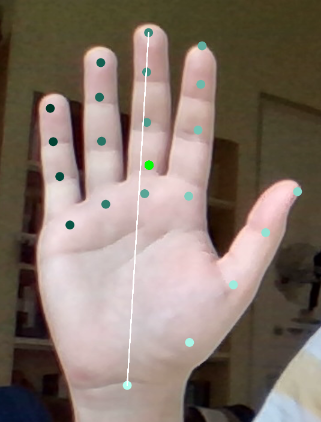
\includegraphics[scale=0.8]{hand.png}
\caption{21 hand points and control parameters}
\end{figure}

From these 21 points (x and y coordinates) we compute 3 parameters:
\begin{itemize}
	\item the centroid (green dot) with coordinates:
	\[x_c = \cfrac{\sum_{i = 1}^{21}x_i}{21}\]
	\[y_c = \cfrac{\sum_{i = 1}^{21}y_i}{21}\]
	\item the distance between the tip of the middle finger $(x_{mf}, y_{mf})$ and the base of the palm $(x_{pb}, y_{pb})$ (length of the white line): 
	\[d = \sqrt{(x_{pb} - x_{mf})^2 + (y_{pb} - y_{mf})^2}\]
	\item the orientation of the hand (the slope of the white line) between $[0, \pi]$:
	\[s = \left\lvert\arctan{\left(\cfrac {y_{mf} - y_{pb}}{x_{mf} - x_{pb}}\right)}\right\rvert \]
\end{itemize}  

 
The user interface is hosted as a web page/application in an Express server, the connection is set up through the framework Socket.io. All the control parameter mentioned above are computed in the client and then sent to the server. From the server, the parameters are written in OSC messages and forwarded to SuperCollider. This last past is handled through the library osc.js, which can generate OSC messages from javascript objects and establish a connection with a receiver (i.e., SuperCollider through an UDP connection). The OSC message has only one path “/params” in which are contained all the parameters as floats.

\begin{figure}[h]
\centering
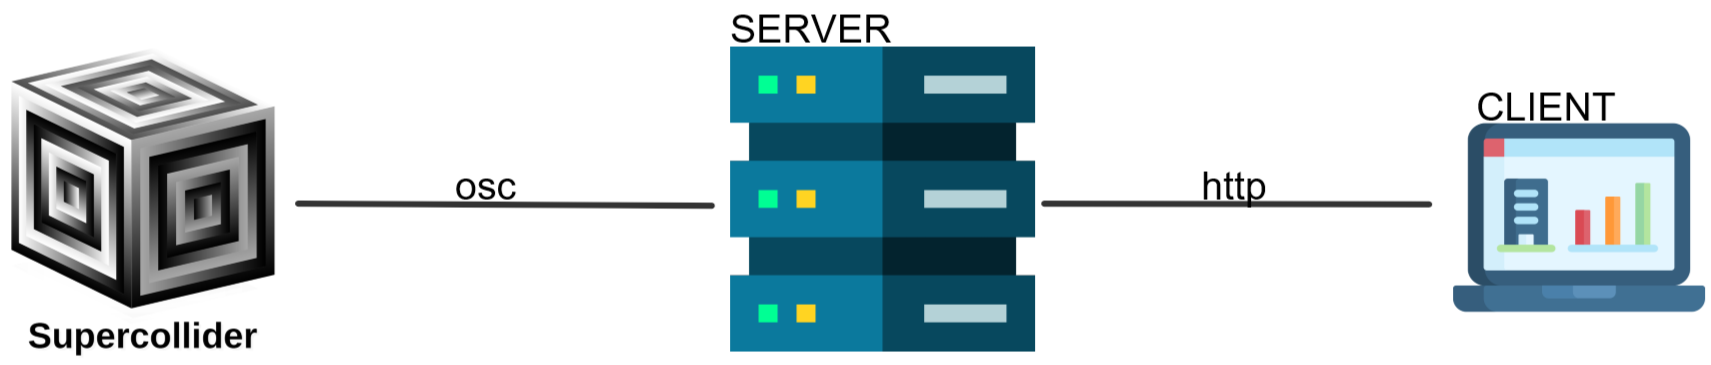
\includegraphics[scale=0.4]{arch.png}
\caption{Application architecture}
\end{figure}


The user interface, as we just said, is a web application in which we imported the libraries ml5.js and p5.js.  We set p5.js in Instance Mode in order to manage 4 different sketches which compose the main window. The bigger p5 sketch at the top left is the one visualizing the webcam, the 21 points of the hand and the control parameters. The other three are a representation of the control parameters using psychedelic animations. At the bottom left we have a visualization for the hand orientation, at the top right for the x and y position of the centroid, and finally at the bottom right, for the distance between the middle finger and the palm base. Going into more depth on the animations implementation, we used as a reference the examples on the \url{https://p5js.org}
website and a number of Youtube tutorials, in order to properly manage all the instructions in the code.\\
\\Beginning from the \textbf{"Squared Rose"} animation, we wanted to create an easily interpretable as visually impactful effect describing the variation of (...). \\The main characteristics of the code itself can be riassumed in the following choices:\begin{itemize}
\item mapping the behaviour of the changing colors with $sin()$ and $cos()$ functions, creating pleasant and smoothing transitions
\item introduce a constant rotation of the figure using the \texttt{rotate} function, and considering as argument \textit{frameCount}, which contains the number of frames that have been displayed since the program started. You can reduce the rotation speed dividing \textit{frameCount} by a proper value. Without this rotation we only have a series of concentric squares, whose relative positions don't change over time.
\end{itemize}
About the \textbf{"Sun Sphere"} animation instead, the astonishing effect given by the cohesion between the central sphere (created with a for cycle of multiple ellipses) and the colorful rays (created with a for cycle of multiple triangles) is essentially possible thanks to the double rotation implemented, through the functions \texttt{rotateX} and \texttt{rotateY}.
The behaviour of the colors is similar to the previous animation, except for the increased velocity in the transitions. This "2 in 1 animation canvas" is used to describe the variations of (...).\\
\\Talking about the \textbf{"Double Square"} animation, we decided to implement an immediately readable effect, describing the variation of (...). The 2 squares gradually decrease \& increase their dimension following the hand orientation, as we'll show in the demo. This effect is given mapping the parameters of the \texttt{rect} functions with the changing positions of the hand over time. In particular, two variables $r1$ and $r2$ (one variable per square) are used for controlling the width and height of the squares in the \texttt{rect} functions. The $r2$ variable depends from $r1$ (actually $r1$ is related to the square on the left) and $r1$ maps the values representing the hand orientation with the width and height of the square: decreasing the width will consequently decrease the height of the first square. In addition, $r1$ and $r2$ are also used for creating a vanish effect while a square is decreasing its size, as arguments of the the two \texttt{fill} functions in the code.


\end{document}
